%% Template for posters

\documentclass[36pt]{sciposter}

\usepackage{preposterTikz} % preamble pakcage

\geometry{paperwidth=90cm,paperheight=100cm,centering,
    textwidth=85cm,textheight=94cm,left=0cm,top=2cm}

\pgfplotsset{compat=1.18}  % 绘图,坐标轴,颜色高级功能都集中在pgfplots包中
%********************************************************************
%********************************************************************

\begin{document}

\onehalfspacing

%%Fill in the commands below with your data.
\newcommand{\titleposter}{JOB TITLE JOB TITLE JOB TITLE}%%titulo do poster
\newcommand{\bigtitle}{JOB TITLE} %%Fill in the parentheses only if the title does not fit on one line.
%%ATTENTION: If you are not going to use the second line, just leave nothing between "{}".
\newcommand{\name}{Surname 1$^{(a)}$, name1, Surname 2$^{(b)}$, name2, Surname 3$^{(b)}$, name3} %%your name
\newcommand{\institutional}{$(a)$ Institution 1, $(b)$. Institution 2} %%institution


%%Title created with TikZ (using \newcommand).
\mytitle{sifsc}{QuadradoBranco}{BoxCol} %blue
%Place the SIICUSP logo in the white square.

\vspace{4cm} 

\section*{\titleA{SUMMARY}}


 
\begin{CJK}{UTF8}{gbsn}
    这是本篇文章的总结和提炼,将说明此文章的目的和受众,指出关键词。AMI系统主要由设备层,通讯层和系统软件层组成。设备层有单相智能电表,三相智能电表,采集器,集中器或AP等组成。通讯方式也有常用的PLC,RF,GPRS/4G等。系统侧有前置机,WEB和数据库组成。
\end{CJK}


%%Text in 2 columns
\begin{multicols}{2}

%%Paragraph.
\setlength{\parindent}{3em}

\section*{\titleA{OBJECTIVES}}

\noindent
 Nullam non leo at mi finibus venenatis. Ut venenatis est in elit varius, quis tincidunt arcu eleifend. In et velit eu elit facilisis faucibus ut sit amet erat


\section*{\titleA{METHODOLOGY}}

Suspendisse diam nisl, mattis nec volutpat sit amet, vestibulum vitae diam. Suspendisse ultrices ac est eu feugiat. Fusce ut efficitur purus. Curabitur suscipit nisi ut fermentum pretium. Suspendisse potenti. Morbi laoreet lobortis nisl, sit amet vulputate lectus porta nec. Vestibulum eget tincidunt nisi. Suspendisse venenatis faucibus massa. Nullam elementum enim eget ante finibus pharetra. Integer porta ipsum id arcu imperdiet tempor. Integer imperdiet commodo urna.
 \begin{equation}
     F = ma \quad\text{texto no meio}\quad \frac{dv}{dt}= \lim_{h\to0} \frac{v(t+h)-v(t)}{h}
 \end{equation}




\section*{\titleA{RESULTS}}


Integer ipsum enim, auctor eget venenatis quis, pellentesque vitae sem. Mauris egestas eleifend dui vitae ornare.

\begin{figure}[h]
\begin{center}
\subfigure[Tetraedro Regular.]{
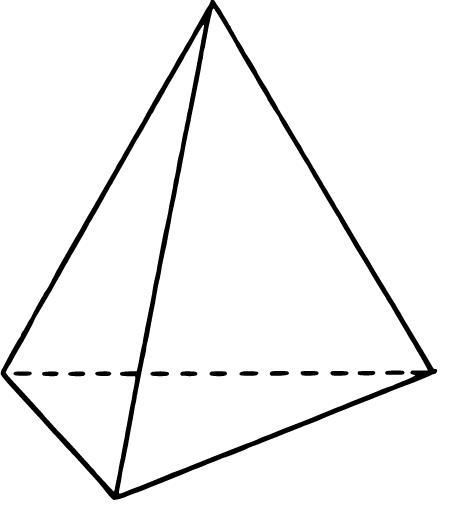
\includegraphics[width = 12cm]{Figuras/Taetraedro_Exemplo.jpg}
}
\subfigure[Molécula de DNA]{

\includegraphics[width = 16.7cm]{Figuras/DNA_Exemplo.jpg}
}
\caption{ example of figures}
\end{center}
\end{figure}

Cras scelerisque suscipit pellentesque. Vivamus accumsan diam at interdum semper. Vivamus vestibulum imperdiet maximus. Cras mollis ultricies leo. Class aptent taciti sociosqu ad litora torquent per conubia nostra, per inceptos himenaeos. Nunc in lobortis enim.

\begin{table}[h!]
    \centering
    \begin{tabular}{|c|c|}
    \hline
         $n$ & Razão entre $a_{n+1}/a_{n}$  \\
    \hline
        $1$ & $1$\\ 
    \hline
         $2$ &  $2$\\
    \hline
        $3$ & $1.5$\\
    \hline
        $4$ & $1.666$\\
        \hline
        $5$ & $1.6$\\
        \hline
    \end{tabular}
    \caption{Razão entre os números da sequência de Fibonacci, onde $a_n$ representa o $n-$ésimo termo.}
\end{table}

Suspendisse imperdiet mollis velit nec tincidunt. Vivamus laoreet nulla non magna hendrerit, non dignissim enim porta. Quisque eget ex odio. Vestibulum non ex mollis, sodales nunc ut, varius quam. Aliquam fringilla convallis nulla.

 Suspendisse diam nisl, mattis nec volutpat sit amet, vestibulum vitae diam. Suspendisse ultrices ac est eu feugiat. Fusce ut efficitur purus. Curabitur suscipit nisi ut fermentum pretium. Suspendisse potenti.



\section*{\titleA{CONCLUSIONS}}

Nullam ex turpis, imperdiet nec maximus eget, placerat id lorem. Fusce lacinia, tellus eget elementum fermentum, velit turpis dapibus enim, tristique posuere augue nibh blandit metus.

\section*{\titleA{REFERENCES}}
\begin{enumerate}
	\item[[1]]\small{SOBRENOME, Nome do autor (abreviado). Título do artigo. Título da Revista, (abreviado ou não) Local, Número do Volume, Número do Fascículo, Páginas inicial-final, mês e ano}
 \end{enumerate}




\section*{\titleA{SUPPORTERS}}

\begin{figure}
    \centering
    
\includegraphics[scale = 0.8]{Figuras/Logos/ifsclogo.png}
    \label{ifsc}
\end{figure}
\begin{minipage}{0.33\linewidth}
\centering
    \begin{figure}[b]
    \centering
    
\includegraphics[width =9cm]{Figuras/Logos/Fapesp.png}

    
    \vspace{0.5cm}
    {\small{Processo 1234567}}
    \end{figure}
\end{minipage}
\begin{minipage}{0.33\linewidth}
\centering
    \begin{figure}[b]
    \centering
    
\includegraphics[width =6cm]{Figuras/Logos/capes.jpg}
    
    
    \vspace{0.5cm}
    {\small{Processo 1234567}}
    \end{figure}
\end{minipage}
\begin{minipage}{0.33\linewidth}
\centering
    \begin{figure}[b]
    \centering
    
\includegraphics[width=12cm]{Figuras/Logos/cnpq.jpg}
    
    \vspace{0.9cm}
    {\small{Processo 1234567}}
    \end{figure}
\end{minipage}



\end{multicols}

\end{document}